\documentclass{article}
\usepackage{v-problem}
\vgeometry
\usepackage{v-electrostatics}

\begin{document}
\vtitle[ELECTROSTATICS]

\def\pn{07}
\def\book{Irodov}
\def\page{106}
\def\gdrive{https://drive.google.com/drive/folders/1i-0I_HCDTkbZh6_rP6Jya5u9xt8flSy3?usp=share_link}

\def\question{
A positive point charge $50\,\upmu\!\Coulomb$ is located in the plane $xy$ at the point with radius vector $\vec{r}_0= 2\hat{i} + 3\hat{j}$, where $\hat{i}$ and $\hat{j}$ are the unit vectors of the $x$ and $y$ axes. Find the
vector of the electric field strength $\vec{E}$ and its
magnitude at the point with radius vector
$\vec{r} = 8\hat{i} - 5\hat{j}$. Here, $r_0$ and $r$ are expressed in
metres.
}

\vspace*{\fill}
\begin{tikzpicture}
	\node[qnumber] (n) at (0, 0)[scale=2] {$\pn.$};
	\node[question] (q) [right=2mm of n.east] {\question};
	\tzline[divider]<-0.125, 0> (q.north west)(q.south west);
	\node[format] (f) at  (q.south east){[\book \quad \page]};
\end{tikzpicture}	
\vspace*{\fill}

\begin{center}
\begin{tikzpicture}
\tzcoor*(0, 0)(O){$O$}[bl]
\tzcoor*(1, 1.5)(r0){$q$}[a](8pt)
\tzcoor*(4, -2.5)(r){}
	\tzaxes(0, -3)(6,3){$x$}{$y$}
	\tzline[-->--=0.95](O)(r0){$\vec{r}_0$}[ma]
	\tzline[->](O)(r){$\vec{r}$}[ma]
	\tzline[-->--=0.5, dashed](r0)(r)
\end{tikzpicture}
\end{center}
\pagebreak

\vtitle[\texttt{Solution}]
\begin{center}
\begin{tikzpicture}
\tzcoor*(0, 0)(O){$O$}[bl]
\tzcoor*(1, 1.5)(r0){$q$}[a](8pt)
\tzcoor*(4, -2.5)(r){}
	\tzaxes(0, -3)(6,3){$x$}{$y$}
	\tzline[-->--=0.95](O)(r0){$\vec{r}_0$}[ma]
	\tzline[->](O)(r){$\vec{r}$}[ma]
	\tzline[-->--=0.5, dashed](r0)(r){$\vec{r}_{rq}$}[mr]
\end{tikzpicture}
\end{center}

\begin{align*}
\vec{v}_0 + \vec{r}_{rq} &= \vec{r}\\
\vec{r}_{rq} &= 8\hat{i}-5\hat{j} - 2\hat{i} - 3\hat{j}\\
\Aboxed{\vec{r}_{rq} &= 6\hat{i}-8\hat{j} }\\
\Aboxed{\left| \vec{r}_{rq}\right| &= 10}
\end{align*}



\begin{align*}
\vec{E} &= \EF\\
		&= \K \dfrac{50\,\upmu\!\Coulomb}{10^2} \dfrac{6\hat{i}-8\hat{j}}{10}\\
		&=9 \times 10^9 \times \dfrac{50 \times 10^{-6}}{10^3} \times \left(6\hat{i}-8\hat{j}\right)\\
		&= 900\left(3\hat{i}-4\hat{j}\right)\\[5mm]
\left|\vec{E}\right| &= 900 \times 5\\
		&= 4.5 \;\text{k}\!\V/\m \ans
\end{align*}

\pagebreak

\vspace*{\fill}
\begin{center}
	\fbox{\qrcode[height=2cm]{\gdrive}}
\end{center}
\vspace*{\fill}

\end{document}
